\chapter{HIL}

\textbf{System name:}  Pendulum with DC Motor
\textbf{List of files:} 
\begin{tabular}{ |c|c| }
    \hline
    main.m & Parameters initialization \\
    model.slx & Main model \\
    \hline
\end{tabular} \\
\textbf{Datasheets:}
\begin{tabular}{ |c|c| }
    \hline
    adxl335.pdf & Accelerometer \\
    lem.pdf & LEM sensor \\
    moc23series.pdf & DC motor \\
    potenc.pdf & Potentiometer \\
    \hline
\end{tabular} \\

\section{Selection and description of the controlled system}
Modeled system is pendulum driven by dc motor, figure \ref{fig:hil_model}
schematically shows the system. 

\begin{figure}[htb!]
    \centering
    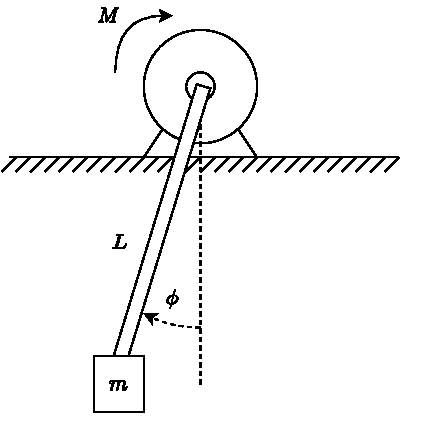
\includegraphics[width=0.5\textwidth]{hil_model.pdf}
    \caption{Pendulum driven by dc motor}
    \label{fig:hil_model}
\end{figure}

System parameters \ref{tab:params}.
\begin{table}[h]
    \centering
    \begin{tabular}{|c|c|c|}
        \hline
        U & 36 & [V] Terminal Voltage \\
        R & 4  & [$\rm\Omega$]  Resistance \\
        L & 5.5e-3  &    [H] Inductance \\
        J & 1.55e-5 &    [kg.m3] Inertia \\
        b & 9.55e-5 &    [Nm/(rad/s)] Damping coefficient \\
        K & .03;    &    [V/(rad/s)] Constant of Proportionality \\
        M & 1024;   & Encoder \\
        I\_max & 10 &    [A] Max current \\
        phi\_max & 2&  [rad] Phi max angle  \\
        m & 200;    &    [g] Mass \\
        l & 0.1;    &   [m] Length \\
        \hline
    \end{tabular}
    \caption{System Parameters}
    \label{tab:params}
\end{table}


\section{Model of a controlled system in Simulink}
Controlled system is DC motor with digital controlled H-bridge
with extinction mechanical pendulum.
\ref{fig:controlled_system}
\begin{figure}[htb!]
    \centering
    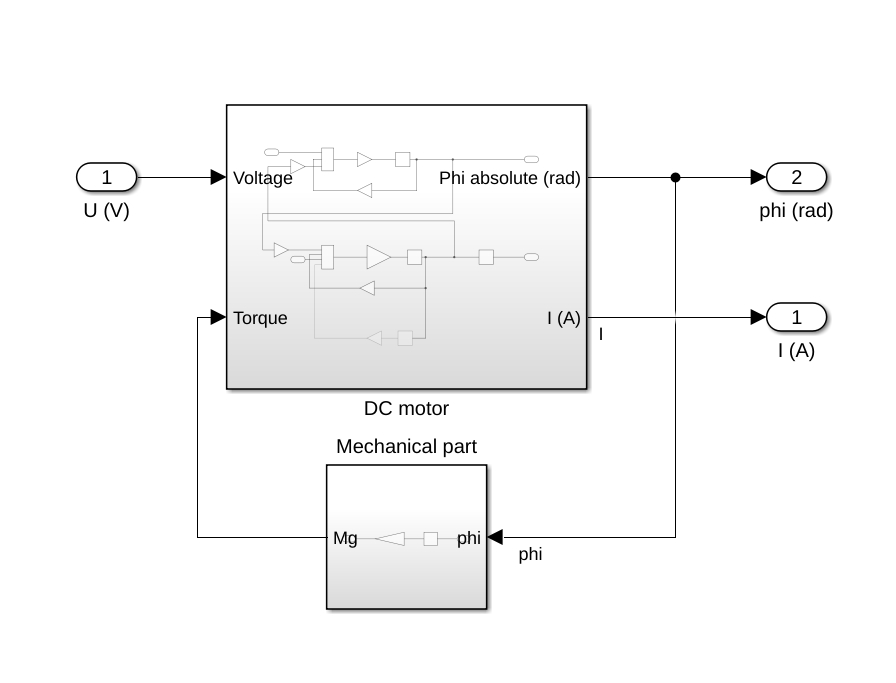
\includegraphics[width=0.6\textwidth]{hil_motor_pendlum.png}
\caption{Controlled system Simulink model}
    \label{fig:controlled_system}
\end{figure}

DC motor with sensors and digital controlled H-bridge is on figure
\ref{fig:motor_sensors}
\ref{fig:controlled_system}
\begin{figure}[htb!]
    \centering
    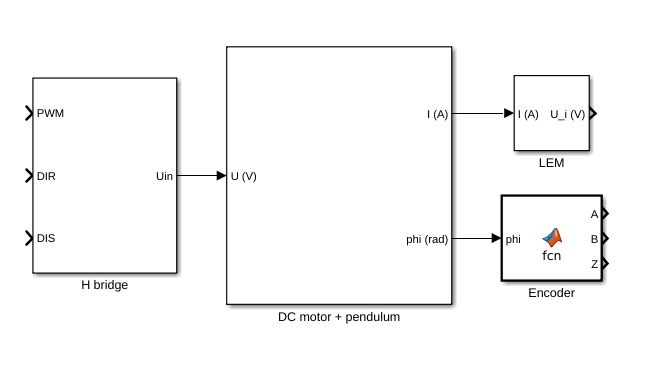
\includegraphics[width=0.6\textwidth]{hil_motor_sensors.png}
\caption{Controlled system Simulink model with sensors}
\label{fig:motor_sensors}
\end{figure}


\section{Models of sensors and actuators}
As a sensors were used encoder with 3 channels A,B and Z measure position
and velocity of dc motor \ref{fig:encoder}. LEM sensor to measure current in dc motor
\ref{fig:lem}.

\begin{figure}[hbt!]
    \centering
    \begin{minipage}{.5\textwidth}
    \centering
    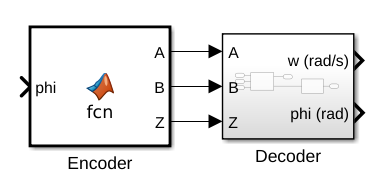
\includegraphics[width=0.6\textwidth]{hil_encoder.png}
    \caption{Encoder sensor}
    \label{fig:encoder}
\end{minipage}%
\begin{minipage}{.5\textwidth}
    \centering
    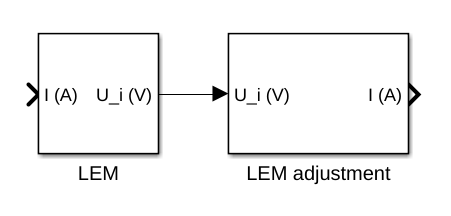
\includegraphics[width=0.5\textwidth]{hil_lem.png}
    \caption{LEM sensor}
    \label{fig:lem}
\end{minipage}
\end{figure}

\section{Control unit and signal adaptation}
Control Unit process encoder position and generate PWM using PID regulator;
LEM sensor control provide motor current protection\ref{fig:control_unit1}.





\begin{figure}[hbt!]
    \centering
    \begin{minipage}{.5\textwidth}
    \centering
    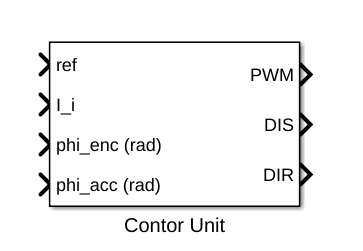
\includegraphics[width=0.5\textwidth]{hil_control_unit.png}
\caption{Control sub-block}
\label{fig:control_unit1}
\end{minipage}%
\begin{minipage}{.5\textwidth}
    \centering
    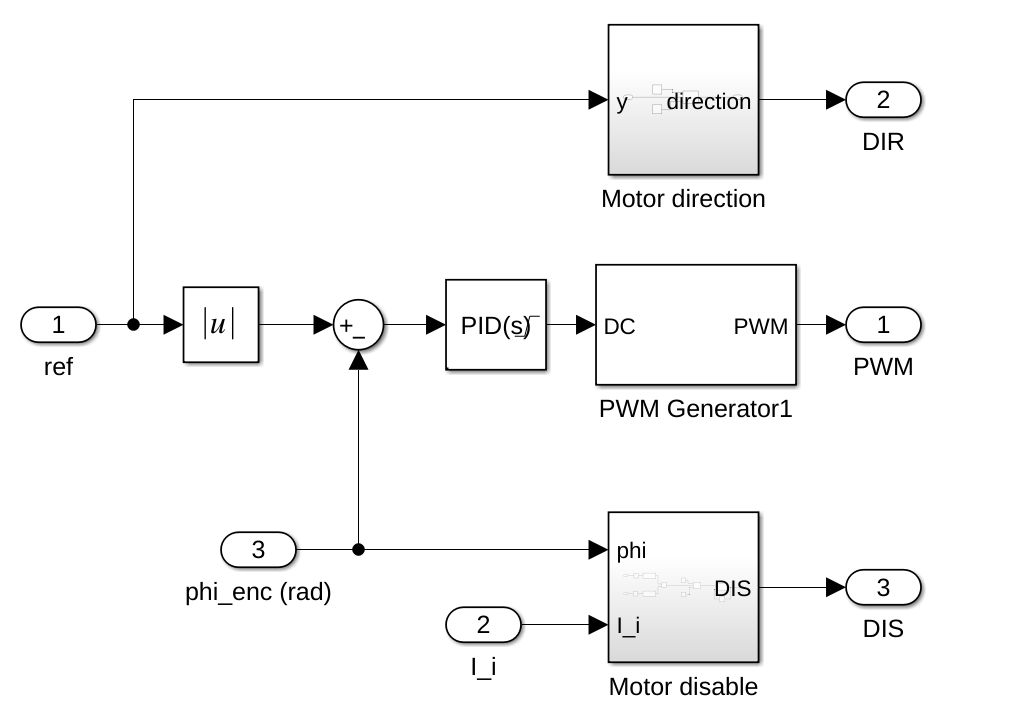
\includegraphics[width=1\textwidth]{hil_control_in.png}
    \caption{Control unit}
    \label{fig:control_unit2}
\end{minipage}
\end{figure}

\section{Tests}

\subsection{Correct Setup}
Correct setup with normal operation conditions. For potentiometer
regulation Simulink knob was used \ref{fig:knob}.  

\begin{figure}[h!]
    \centering
    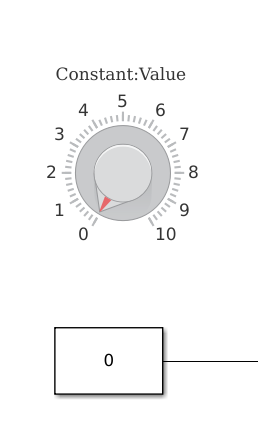
\includegraphics[width=0.15\textwidth]{hil_potenciometer_gui.png}
    \caption{Potentiometer regulation knob}
    \label{fig:knob}
\end{figure}


\begin{figure}[htb!]
    \centering
    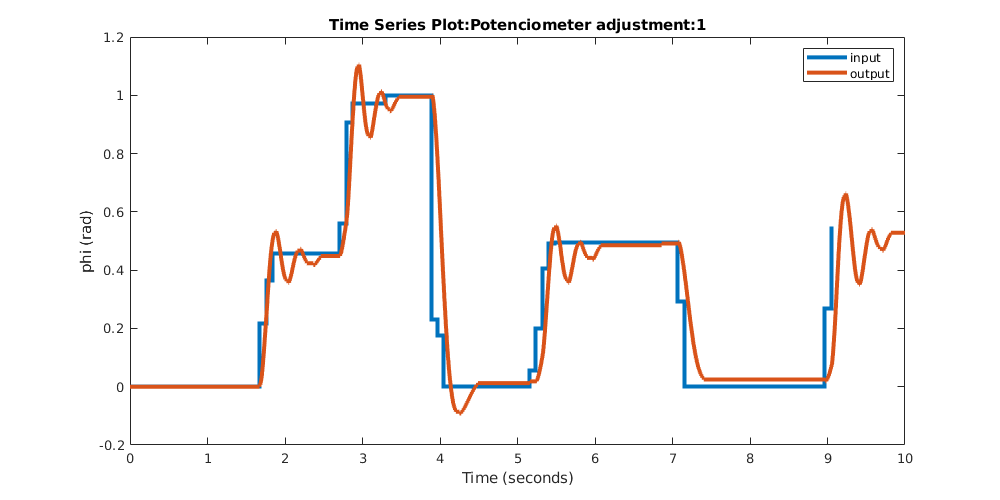
\includegraphics[width=0.7\textwidth]{hil_normal.png}
\caption{Correct setup test}
    \label{fig:correct}
\end{figure}

\subsection{Changing Pendulum Parameters}
Pendulum length parameter changing from $l = 0.1 \rm\  [m]$ to
$l = 0.2 \rm\  [m]$. Result system behavior  (fig. \ref{fig:change}.

\begin{figure}[htb!]
    \centering
    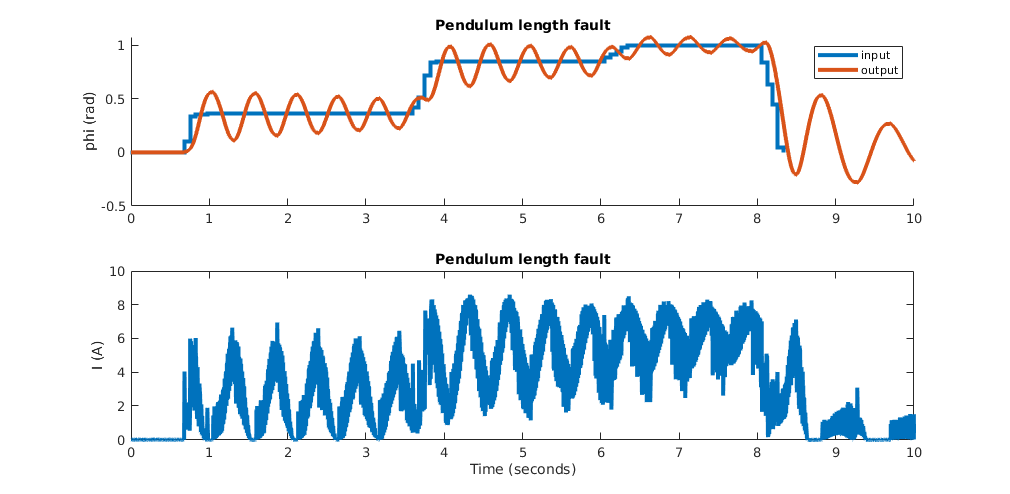
\includegraphics[width=0.7\textwidth]{hil_pendulum_fault.png}
\caption{Changing parameters test}
    \label{fig:change}
\end{figure}

\subsection{Encoder Resolution Fault}
Encoder fault is given by decreasing encoder resolution from  1024 cycle to 
512 cycles \ref{fig:encoder_fault}.
\begin{figure}[htb!]
    \centering
    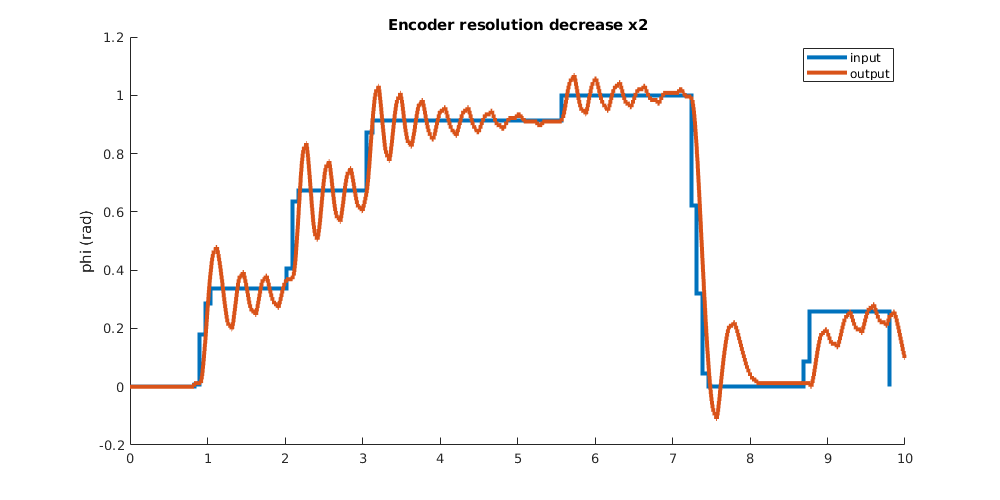
\includegraphics[width=0.7\textwidth]{hil_encoder_fault.png}
\caption{Encoder resolution fault}
    \label{fig:encoder_fault}
\end{figure}

\newpage
\subsection{Encoder B channel fault}
After encoder channel B was disconnected the system has no longer right
position information \ref{fig:encoder_B}
\begin{figure}[h!]
    \centering
    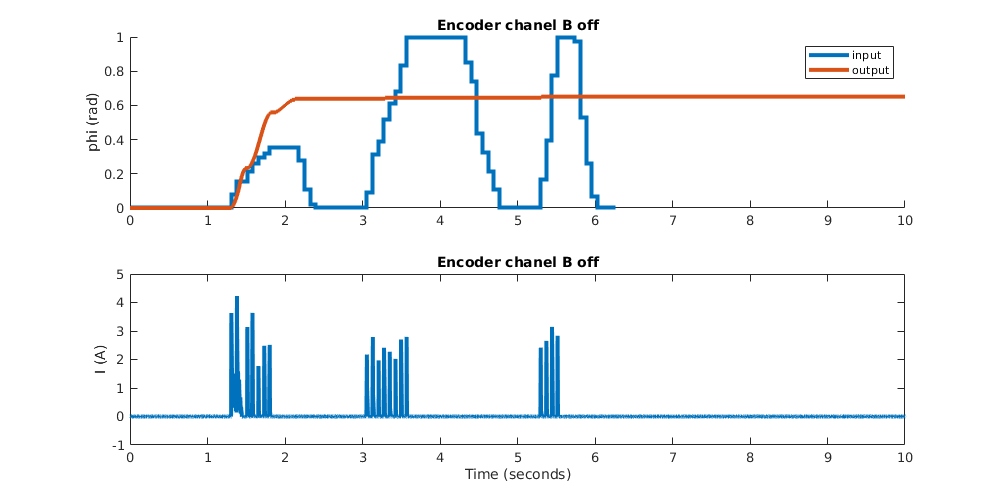
\includegraphics[width=0.7\textwidth]{hil_chanel_B.png}
    \caption{Encoder B channel fault}
    \label{fig:encoder_B}
\end{figure}

\subsection{Current Protection lower value}
If we change current protection threshold to lower value from 10 to  7 A. The
control unit will immediately stop dc motor \ref{fig:current}.
\begin{figure}[h!]
    \centering
    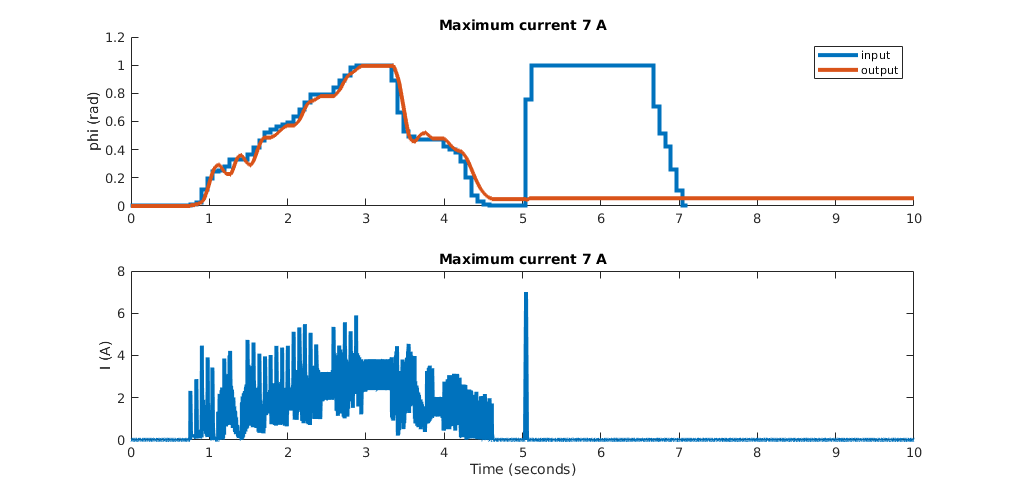
\includegraphics[width=0.7\textwidth]{hil_max_current.png}
    \caption{Current Protection}
    \label{fig:current}
\end{figure}



\subsection{Noisy Input from Potentiometer}
In this situation noisy signal from input potentiometer was modeled
\ref{fig:poten_fault}.
\begin{figure}[h!]
    \centering
    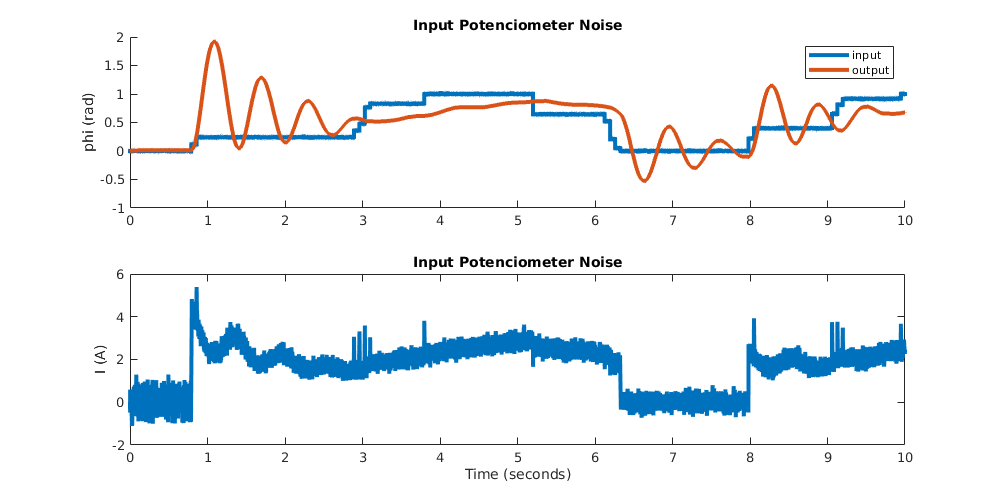
\includegraphics[width=0.7\textwidth]{hil_input_noise.png}
    \caption{Noisy Potentiometer}
    \label{fig:potent_fault}
\end{figure}



\section{Evaluation of the whole task and conclusion}
The DC motor with a pendulum was modeled as a controlled system. PID
controller was used as a regulator. The plant was extended by sensors and
digital control H-bridge. Using the control unit, position regulation by a
potentiometer and current protection was implemented and tested as a HIL
object. All used parameters were extracted from included datasheets.


